% !TeX spellcheck = si_SI
\newpage
\chapter{Rezultati in diskusija}\label{cha:rezultati}

    Prikažemo lahko sposobnost vibroizolacije numerične analize primera metamateriala definiranem v poglavju \ref{sec:zasnova_MM_verige}. 
    V primerjavi na grafu $\abs{T(f)}$ \ref{fig:prenosna_funkcija_MM} vidimo, da se tako direktna metoda z numerično integracijo in indirektna metoda z linearizacija dobro ujemata. Opazimo lahko obstoj pasovne vrzeli v območju med $2$ in $3$ Hz. Tam se zaradi prisotnosti zavrnitvenega pasu vibracije ne prenašajo. 
    
    \begin{figure}[!hb]
        \centering
        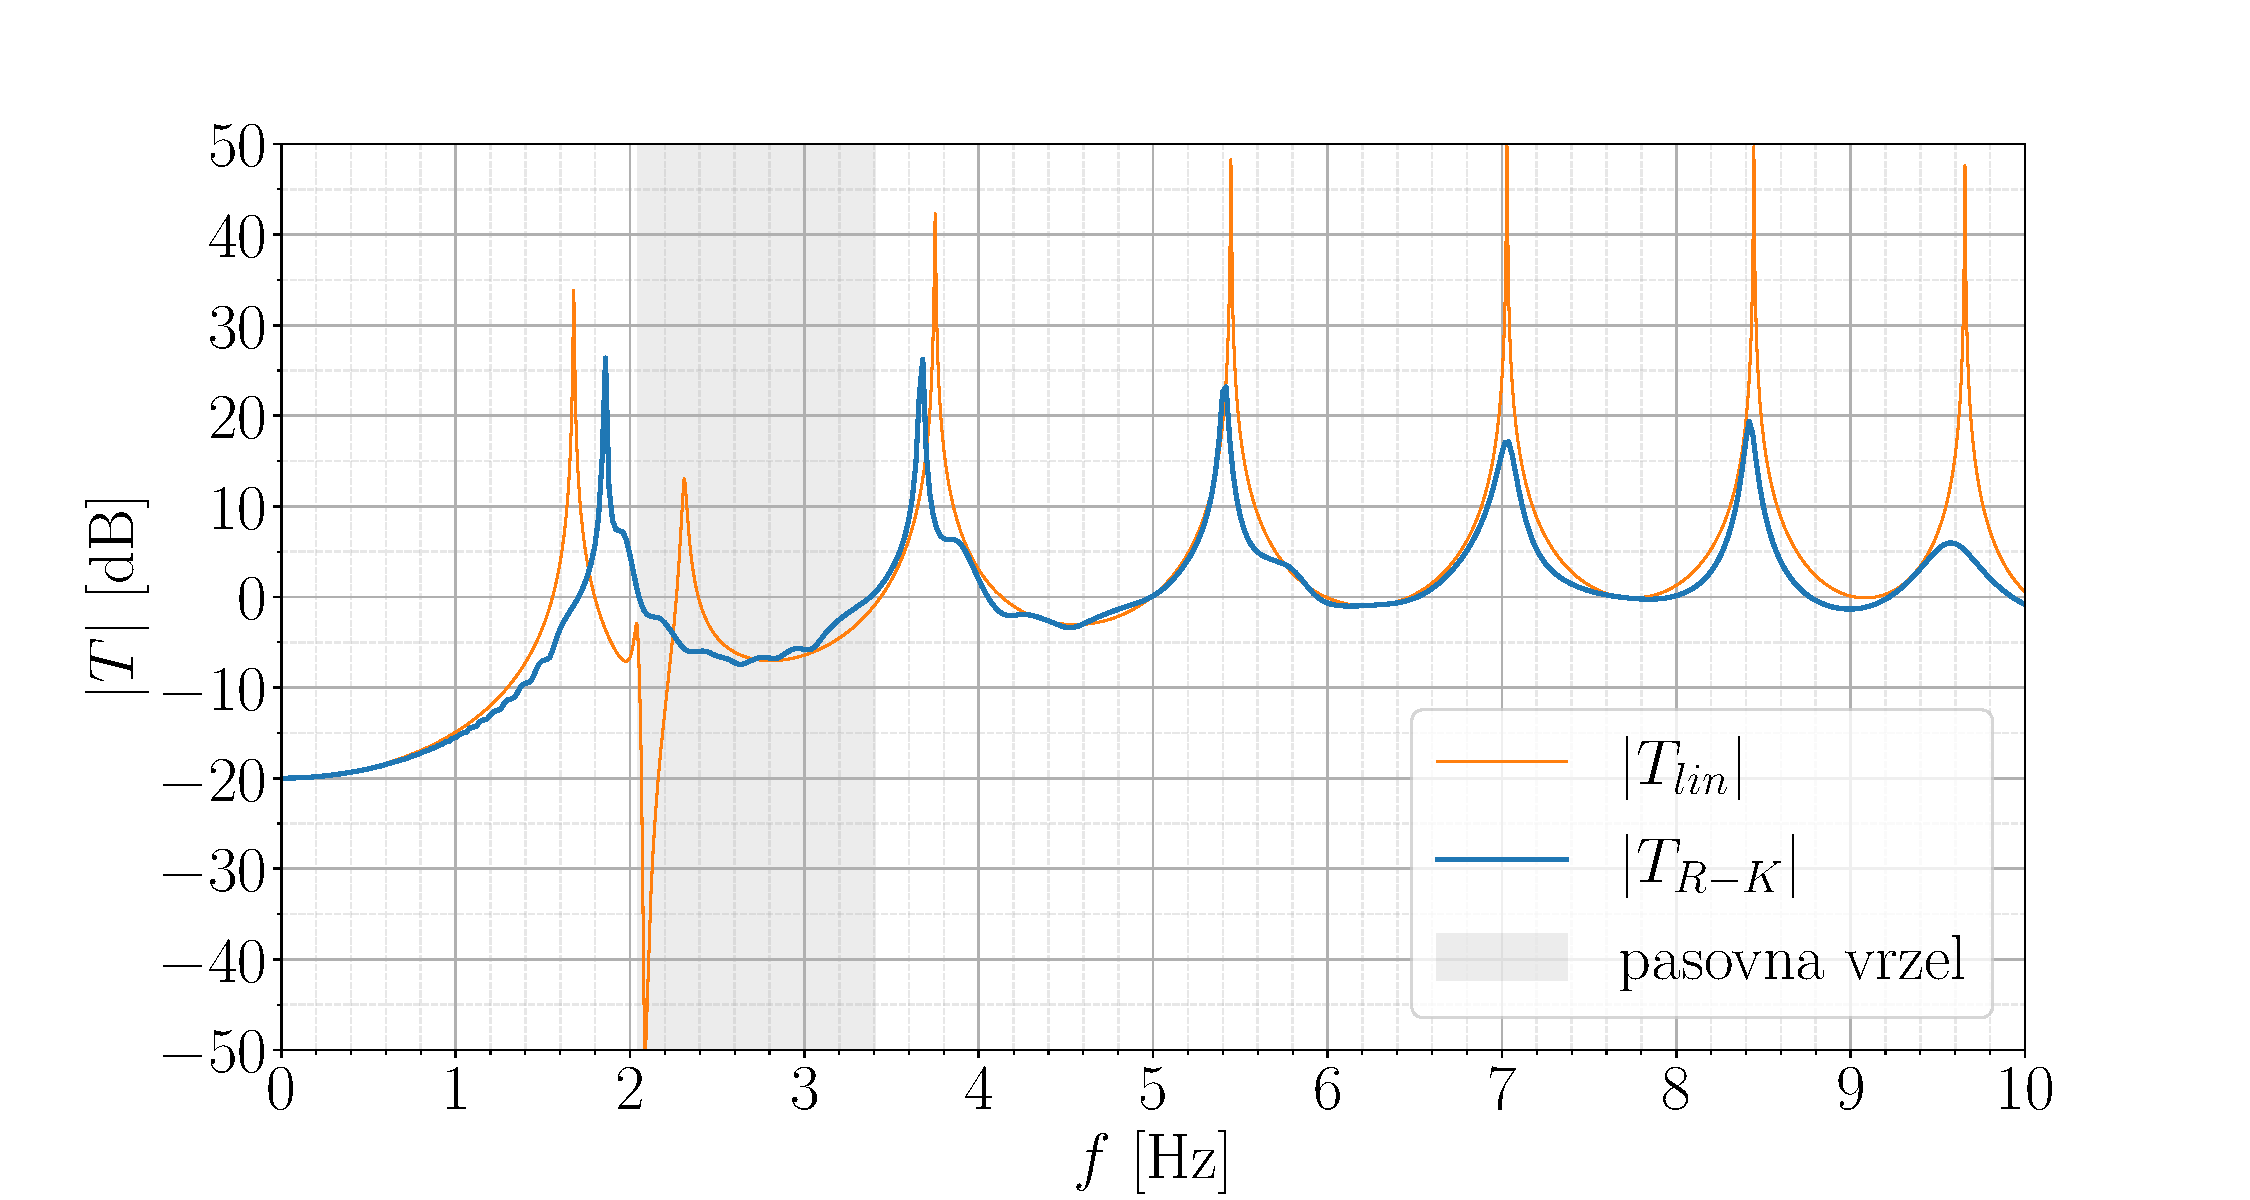
\includegraphics[trim={0.0cm 0.0cm 0.0cm 1.0cm}, clip, scale=0.45]{Magisterski praktikum/slike/rezultati/FRF_Abs_numerika.pdf}
        \caption{Prenosnost pomika pri različnih frekvencah.}\label{fig:prenosna_funkcija_MM}
    \end{figure}

     Iz enačbe \ref{eq:disperzijska_krivulja} vidimo, da je delovanje metamateriala odvisno predvsem od dušilnega razmerja $\zeta$, masnega razmerja $\beta$ in razmerja togosti ter predvsem nelinearne togosti $\alpha$. S slike \ref{fig:FRF_disperzijska} lahko vidimo, da se z večanjem togosti pasovna vrzel pomika proti višjim frekvencam, pri višanju dušenja pa se pasovna vrzel širi, vendar je pri tem manj učinkovita.  

     Zaradi občutljivosti modula elastičnosti $E_{GPLA}$ na temperaturo, je dejanska prenosnost funkcija temperature $T=T(f, \text{temp.})$.